% !TEX TS-program = XeLaTeX
% use the following command:
% all document files must be coded in UTF-8
\documentclass[portuguese]{textolivre}
% build HTML with: make4ht -e build.lua -c textolivre.cfg -x -u article "fn-in,svg,pic-align"

\journalname{Texto Livre}
\thevolume{18}
%\thenumber{1} % old template
\theyear{2025}
\receiveddate{\DTMdisplaydate{2024}{12}{26}{-1}} % YYYY MM DD
\accepteddate{\DTMdisplaydate{2025}{3}{11}{-1}}
\publisheddate{\DTMdisplaydate{2025}{6}{9}{-1}}
\corrauthor{Glauber de Souza Lemos}
\articledoi{10.1590/1983-3652.2025.56730}
%\articleid{NNNN} % if the article ID is not the last 5 numbers of its DOI, provide it using \articleid{} commmand 
% list of available sesscions in the journal: articles, dossier, reports, essays, reviews, interviews, editorial
\articlesessionname{dossier}
\runningauthor{Lemos e Desidério} 
%\editorname{Leonardo Araújo} % old template
\sectioneditorname{Hugo Heredia Ponce}
\layouteditorname{Daniervelin Pereira}

\title{Tradução de texto-escrito escolar de geografia para texto-vídeo: criatividade nos usos de imagens e descrições imagéticas da sinalização em libras}
\othertitle{Translating a Geography school text into a video text in Brazilian Sign Language (Libras): creativity in the use of images and imagetic descriptions}
% if there is a third language title, add here:
%\othertitle{Artikelvorlage zur Einreichung beim Texto Livre Journal}

\author[1]{Glauber de Souza Lemos~\orcid{0000-0001-5907-1653}\thanks{Email: \href{mailto:glauberlemos@letras.ufrj.br}{glauberlemos@letras.ufrj.br}}}
\author[2]{Rosemeire Aparecida Antunes Desidério~\orcid{0009-0005-7363-0577}\thanks{Email: \href{mailto:rosea@unicamp.br}{rosea@unicamp.br}}}
\affil[1]{Universidade Federal do Rio de Janeiro, Faculdade de Letras, Departamento de Letras-Libras, Rio de Janeiro, RJ, Brasil.}
\affil[2]{Universidade Estadual de Campinas, Faculdade de Ciências Médicas, Centro de Estudos e Pesquisas em Reabilitação, Campinas, SP, Brasil.}

\addbibresource{article.bib}
% use biber instead of bibtex
% $ biber article

% used to create dummy text for the template file
%\definecolor{dark-gray}{gray}{0.35} % color used to display dummy texts
%\usepackage{lipsum}
%\SetLipsumParListSurrounders{\colorlet{oldcolor}{.}\color{dark-gray}}{\color{oldcolor}}

% used here only to provide the XeLaTeX and BibTeX logos
%\usepackage{hologo}

% if you use multirows in a table, include the multirow package
\usepackage{multirow}

% provides sidewaysfigure environment
%\usepackage{rotating}

% CUSTOM EPIGRAPH - BEGIN 
%%% https://tex.stackexchange.com/questions/193178/specific-epigraph-style
% \usepackage{epigraph}
% \renewcommand\textflush{flushright}
% \makeatletter
% \newlength\epitextskip
% \pretocmd{\@epitext}{\em}{}{}
% \apptocmd{\@epitext}{\em}{}{}
% \patchcmd{\epigraph}{\@epitext{#1}\\}{\@epitext{#1}\\[\epitextskip]}{}{}
% \makeatother
% \setlength\epigraphrule{0pt}
% \setlength\epitextskip{0.5ex}
% \setlength\epigraphwidth{.7\textwidth}
% CUSTOM EPIGRAPH - END

% to use IPA symbols in unicode add
%\usepackage{fontspec}
%\newfontfamily\ipafont{CMU Serif}
%\newcommand{\ipa}[1]{{\ipafont #1}}
% and in the text you may use the \ipa{...} command passing the symbols in unicode

% LANGUAGE - BEGIN
% ARABIC
% for languages that use special fonts, you must provide the typeface that will be used
% \setotherlanguage{arabic}
% \newfontfamily\arabicfont[Script=Arabic]{Amiri}
% \newfontfamily\arabicfontsf[Script=Arabic]{Amiri}
% \newfontfamily\arabicfonttt[Script=Arabic]{Amiri}
%
% in the article, to add arabic text use: \textlang{arabic}{ ... }
%
% RUSSIAN
% for russian text we also need to define fonts with support for Cyrillic script
% \usepackage{fontspec}
% \setotherlanguage{russian}
% \newfontfamily\cyrillicfont{Times New Roman}
% \newfontfamily\cyrillicfontsf{Times New Roman}[Script=Cyrillic]
% \newfontfamily\cyrillicfonttt{Times New Roman}[Script=Cyrillic]
%
% in the text use \begin{russian} ... \end{russian}
% LANGUAGE - END

% EMOJIS - BEGIN
% to use emoticons in your manuscript
% https://stackoverflow.com/questions/190145/how-to-insert-emoticons-in-latex/57076064
% using font Symbola, which has full support
% the font may be downloaded at:
% https://dn-works.com/ufas/
% add to preamble:
% \newfontfamily\Symbola{Symbola}
% in the text use:
% {\Symbola }
% EMOJIS - END

% LABEL REFERENCE TO DESCRIPTIVE LIST - BEGIN
% reference itens in a descriptive list using their labels instead of numbers
% insert the code below in the preambule:
%\makeatletter
%\let\orgdescriptionlabel\descriptionlabel
%\renewcommand*{\descriptionlabel}[1]{%
%  \let\orglabel\label
%  \let\label\@gobble
%  \phantomsection
%  \edef\@currentlabel{#1\unskip}%
%  \let\label\orglabel
%  \orgdescriptionlabel{#1}%
%}
%\makeatother
%
% in your document, use as illustraded here:
%\begin{description}
%  \item[first\label{itm1}] this is only an example;
%  % ...  add more items
%\end{description}
% LABEL REFERENCE TO DESCRIPTIVE LIST - END


% add line numbers for submission
%\usepackage{lineno}
%\linenumbers

\usepackage{needspace}

\begin{document}
\maketitle

\begin{polyabstract}
\begin{abstract}
Esta pesquisa apresenta uma proposta de tradução de português para língua brasileira de sinais (libras) a respeito de um texto de atividades agrícolas, incluído em um livro didático-escolar de geografia correspondente ao 4º ano do ensino fundamental, ou seja, crianças entre nove e dez anos de idade. O embasamento teórico está fundamentado na linguística das línguas de sinais, na descrição imagética da libras e na tradução intersemiótica. Os resultados da pesquisa apontam que é possível propor uma tradução de geografia em texto-vídeo em libras, mas com usos de elementos descritivos visuais-imagéticos de línguas de sinais, tais como as transferências de tamanho/forma, espaço, localização, movimento e incorporação. E, por fim, observamos que as descrições imagéticas, quando aplicadas na tradução em libras, permitem deixar a sinalização mais icônica-visual, criativa e atrativa para os alunos surdos, aproximando, ainda, os sentidos, os conceitos e as imagens referentes ao texto-fonte de geografia no texto-vídeo em libras.

\keywords{Descrição imagética na libras \sep Texto de geografia em libras \sep Tradução criativa e intersemiótica \sep Tradução em texto-vídeo}
\end{abstract}

\begin{english}
\begin{abstract}
This study presents a proposal for the translation from Brazilian Portuguese into Brazilian Sign Language (Libras) of a text on agricultural activities that is included in a Geography textbook for the fourth grade of primary school (4th grade elementary school; grade K-5), i.e. for children between the ages of nine and ten. The theoretical framework draws on sign language linguistics, Libras’ imagetic description and intersemiotic translation. The results of the study show that it is possible to propose a video text translation of a geography text in Libras, provided that visual-imagetic descriptive elements of sign languages, such as transfers of size/shape, space, location, movement and incorporation are used. And finally, we observed that imagetic descriptions, when applied in the translation into Libras, make the production more iconic, visual, creative and attractive for deaf students, bringing together the meanings, concepts and images referring to the Geography source text in the video text in Libras.

\keywords{Imagetic description in Brazilian Sign Language (Libras) \sep Geography school text in Brazilian Sign Language (Libras) \sep Creative and intersemiotic translation \sep Translation into video text}
\end{abstract}
\end{english}
% if there is another abstract, insert it here using the same scheme
\end{polyabstract}

\section{Introdução}\label{sec-intro}
No início do século XXI, com a publicação da Lei nº 10.098/2000, conhecida como a “lei da acessibilidade comunicacional”, reconhece que os cidadãos surdos se comunicam por meio da Língua Brasileira de Sinais (libras) e, por isso, as instituições devem garantir que estes cidadãos recebam as informações por meio de sua primeira língua (L1). No Brasil, a comunidade surda e seus aliados conquistaram diversas políticas linguísticas, educacionais e sociais, por meio de outras leis nacionais, por exemplo: o reconhecimento da libras como língua circulante no Brasil; a inclusão da disciplina da libras em contexto acadêmico; a obrigatoriedade da inserção e atuação de Tradutores-Intérpretes de Libras-Português (TILSP) e Guia-Intérpretes para Surdocegos (GIS) em diversos contextos e em instituições/empresas públicas e privadas; as recomendações e exigências para a construção de escolas bilíngues para surdos, com foco em uma educação bilíngue (libras como língua de instrução e aquisição linguística dos alunos surdos, além de ensino do português escrito, sendo ensinado como segunda língua), com atuação de professores (surdos e ouvintes) e outros profissionais educacionais bilíngues. 

Certamente, a tradução de materiais escolares em libras é um bem material nacional, pois proporciona conhecimentos, circulações de saberes e informações para os surdos brasileiros. Os autores \textcite{rodrigues2018interpretacao} afirmam que os TILSP vêm atuando, por exemplo, em ambientes escolares e acadêmicos, atendendo as demandas de tradução e interpretação de línguas de sinais para os alunos surdos. No entanto, principalmente na Educação Básica, em escolas inclusivas, a maioria dos alunos surdos possuem pouca acessibilidade linguística aos conteúdos traduzidos de português para libras. No que tange à tradução de materiais didáticos escolares, destacando, aqui, a temática de “geografia”, há poucas produções e/ou falta de acessibilidade para a libras. Há, ainda, poucos ou quase nenhum livro didático escolar traduzido de português para libras, em todos os níveis escolares e acadêmicos. Podemos afirmar isto, pois há poucas publicações acadêmicas que tematizam a tradução de textos escolares em libras \cite{galasso2018materiais,silva2020materiais,baalbaki2024acessibilidade} e quase nenhuma pesquisa focando em tradução de textos de geografia de português para libras. 

Assim sendo, nos questionamos: como é possível traduzir e construir um texto-vídeo de geografia em libras, contendo elementos de descritores imagéticos para os alunos surdos, com idade entre nove e dez anos, cursando o 4º ano do ensino fundamental I? Por conta desta pergunta, referente à área de tradução de textos escolares em libras, a nossa pesquisa se envereda, com os objetivos de construir uma tradução de texto de geografia em língua de sinais e verificar quais elementos linguísticos e imagéticos podem permitir que o texto-vídeo se torne mais significativo para os alunos surdos. Por isso, selecionamos um texto escolar de geografia, tematizando a agricultura agropecuária e os trabalhos rurais, com foco em uma tradução criativa e intersemiótica. 

Acreditamos que mais estudos e pesquisas sobre tradução de textos de geografia em libras precisam ser ampliados, pois trarão luz à ciência geográfica e, consequentemente, benefícios didáticos e escolares aos alunos surdos, fomentando que este público-alvo possa adquirir novos conhecimentos de geografia e, também, colocar em prática o que aprenderam no contexto escolar em sua vida social. 

A seguir, apresentamos, brevemente, os estudos linguísticos das línguas de sinais e a conceituação de iconicidade e descrição imagética da libras. Em seguida, conceituaremos a tradução intersemiótica e a relacionaremos com a tradução em libras e como criatividade visual-espacial. Depois, revistamos as publicações acadêmicas, tematizando a tradução de materiais escolares e acadêmicos em libras. Logo após, analisamos os dados deste estudo, com comentários da tradução feita em texto-vídeo em libras, referente a um texto escolar de geografia para alunos do quarto ano do ensino fundamental I. Por fim, finalizamos o artigo e apresentamos as referências da pesquisa.

\section{Linguística das línguas de sinais, iconicidade e descrição imagética}\label{sec-normas}
A Linguística é uma disciplina acadêmica que estuda as línguas humanas, a partir de sua forma-estrutura-conteúdo e/ou de seu uso funcional-social, observando, descrevendo e analisando os aspectos fonéticos, morfológicos, sintáticos, semânticos, como também com foco analítico discursivo-pragmático e cognitivo-psicolinguístico a respeito das relações entre língua, texto, leitura, cognição, contexto e situação social \cite{petter2002linguagem,bagno2014lingua}. 

As línguas de sinais são diferentes das línguas orais, um exemplo é a relação que se faz na articulação entre os elementos fonoarticulatórios e que são produzidos pelos sons, no caso das línguas orais, que formam palavras, já as línguas de sinais se articulam com os dedos, mãos, cabeça e outros pontos do corpo \cite[p.~11-12]{quadros2025introducao}. No âmbito das línguas de sinais, na década de 1960, o linguista americano William Stokoe descreveu a \textit{American Sign Language} (ASL), afirmando, já nesse período, que era uma língua visual-espacial, contendo fonemas produzidos pelas mãos e com um sistema linguístico complexo, assim como todas as línguas orais. Ou seja, a pesquisa de Stokoe já apontava que havia diferenças de modalidades linguísticas: as línguas orais são articuladas e produzidas de modo oral-vocal-auditivo; e as línguas de sinais são produzidas de modo espacial-gestual-visual. Mais adiante, a partir da década de 1980, outras pesquisas analisaram e comprovaram todos os níveis linguísticos das línguas de sinais (em relação aos níveis fonológicos, morfológicos, sintáticos e semânticos). 

No âmbito dos estudos linguísticos das línguas de sinais, destacamos o nível morfológico e que interessa ao nosso estudo. Isso porque a morfologia possui muitas categorias e aspectos, mas para esta pesquisa, interessa-nos observar os usos de Descrições Imagéticas, no entanto, com foco mais semiótico, em sua interpretação \cite{campello2008visualidade}. Segundo \textcite[p. 92-94]{quadros2004libras} e \textcite[p. 87-100]{castro2012}, os classificadores fazem parte de léxicos dos participantes das comunidades surdas, ou seja, em cada uma das línguas de sinais há criações e incorporações representativas sobre as suas perspectivas, as suas realidades e os seus contextos. Os classificadores sinalizados são integrados no núcleo lexical dos sinais, mas podem não obedecer às regras formacionais-gramaticais morfofonológicas da língua (por exemplo, podem desobedecer às regras de simetria e dominância dos sinais e das mãos). Os classificadores possibilitam que os sinalizantes construam a concordância na sinalização, descrevendo, iconicamente, as pessoas, os animais e os objetos, além de indicar a movimentação, a localização e os formatos. E, também, os classificadores especificam as qualidades de um referente no enunciado sinalizado; predicalizam e dão formas aos objetos na sinalização; modelam as mudanças lexicais dos sinais; e demandam interpretação semântica e contextual para serem compreendidos \cite{quadros2004libras,castro2012}. Os tipos de classificadores em libras são: 
\begin{itemize}
    \item Classificador Descritivo (CL-D)
    \item Classificador Especificador (CL-ESP)
    \item Classificador de Partes do Corpo (CL-PC)
    \item Classificador Locativo (CL-L)
    \item Classificador Semântico (CL-S)
    \item Classificador Instrumental (CL-I)
    \item Classificador de Corpo (CL-C)
    \item Classificador Plural (CL-P)
    \item Classificador de Número ou Nome (CL-N)
\end{itemize}

Nas pesquisas realizadas por \textcite[p.~156]{campello2008visualidade} argumenta-se que o uso da denominação “classificador” ou “classificadores manuais”: (i) podem provocar o “desaparecimento da visualidade e da imagem das línguas de sinais”; (ii) não dão conta de todos os recursos visuais e toda a complexidade linguística espacial-visual das línguas de sinais; (iii) estão fortemente atreladas ao estruturalismo restritivo da iconicidade; e (iv) podem não descrever os conceitos das imagens na sinalização. Assim, \textcite{campello2008visualidade} aponta que a denominação “classificadores” não contempla a linguagem-em-uso das línguas de sinais, ou seja, a denominação de “classificador” é oriunda de um conceito da língua oral e de modalidade falada-escrita, cuja palavra ou afixo pode ser interpretado somente para “classificar” apenas a um substantivo, além de poder depender de algum tipo de referente, por exemplo, a palavra “pedaço” em frases como “três pedaços de doce”.  Portanto, \textcite{campello2008visualidade} defende a denominação de “descrição imagética”, para, assim, contemplar a realidade icônica e imagética das línguas de sinais. Vale relembrar que o aprofundamento desta perspectiva linguística das línguas de sinais surgiu nos Estados Unidos, na University Gallaudet, sendo denominada de \textit{Descriptive Visual}, a partir das pesquisas de Deborah Chen Pichler.

Para \textcite{campello2008visualidade}, o processo de iconização em Libras, com base teórica nos estudos de Iconicidade Cognitiva, constrói-se as transferências de significados literais (formas, tamanhos, situações, pessoas, animais), com foco em produções de realidades imagéticas da sinalização, em determinado espaço-visual e de forma tridimensional. Nas pesquisas empreendidas por \textcite{taub2001language}, para se criar/produzir um item icônico é preciso selecionar uma imagem, depois disso, esquematizá-la e, por fim, modificá-la \cite[p.~50-51]{kogut2015signwriting} – na afirmação de \textcite{campello2008visualidade}, a última etapa é o processo de transferência imagética na produção da sinalização. As descrições imagéticas em línguas de sinais, segundo \textcite{campello2008visualidade}, são propostas mais minimalistas e focadas nos estudos de visualidade e da semiótica. Já a conceituação de descrição imagética se baseia na constituição da forma e em como se sinalizada determinadas especificidades imagéticas para se materializar e incorporar em sinais, dando, assim, mais vida e expressividade aos conceitos e signos linguísticos visuais nas línguas de sinais.

Assim, as Descrições Imagéticas são transferências de percepções visuais, ou seja, um sinalizador pode utilizar as Descrições Imagéticas, com foco em poder descrever objetos, formas, tamanhos e volumes em seu corpo-texto-sinalizador. As cinco Descrições Imagéticas, propostas por Campello, são apresentadas na \Cref{tbl1}.

\begin{table}[htbp]
\caption{Descritores Imagéticos em Libras.}
\label{tbl1}
\centering
\footnotesize
\begin{tabular}{p{4cm} p{10cm}}
\toprule
Descritor imagético & Conceituação \\ 
\midrule
Transferência de Tamanho e de Forma (TTF) & 
\begin{itemize}\vspace{-7pt}
    \item Sinalizada com foco icônico de um signo visual, servindo como representação do tamanho, podendo ser: grande, alto, comprido; agudo; menor, pouco extenso, pouco volume; fino, pequeno, miúdo, estatura abaixo da média; maior, colosso, avantajado; vasto, de longa extensão, longo.
    \item As formas podem ser transferidas de acordo com as características físicas dos seres e das coisas como decorrência da estruturação de suas partes, por exemplo: forte, intenso, violento (dependendo do envolvimento sentimental), poderoso, notável, marcante, acanhado, mesquinho, insignificante, humildade, inferioridade, medroso.
\end{itemize}  \\ 
Transferência Espacial (TE) & 
\begin{itemize}\vspace{-7pt}
    \item Apresenta uma regularidade espacial (para baixo ou cima), podendo ser transferida na sinalização em diferentes ângulos e movimentar-se ou não circularmente.
    \item Podem ser sinalizados em espaços encurvados, curvilíneos, quadrados, retangulares e triangulares.
\end{itemize} \\
Transferência de Localização (TL) & 
\begin{itemize}\vspace{-7pt}
    \item Referencia-se a um determinado lugar da sinalização. 
    \item Marcação da sinalização ou olhar para um espaço ou uma localização.
    \item Sinalizada para uma direcionalidade e que vai para frente e/ou atrás, do lado direito e/ou esquerdo, com alternância de puxar e/ou soltar, com distância ou proximidade.
\end{itemize} \\
Transferência de Movimento (TM) & 
\begin{itemize}\vspace{-7pt}
    \item Serve para se conseguir o equilíbrio visual, mantando a coerência, os opostos, as igualdades e o contrastes na sinalização.
    \item É sinalizado de várias maneiras, por exemplo, como diferenciação entre uma imagem simples ou complexa (inúmeros signos que cobrem um campo inteiro) e como similaridade duas imagens. 
    \item Outro exemplo é de uma apresentação de sinalização a respeito de um contexto, diferenciando-o como por exemplo na condição de ser rico x pobre.
\end{itemize} \\
Transferência de Incorporação (TI) & 
\begin{itemize}\vspace{-7pt}
    \item Esta estrutura reproduz várias ações de pessoas ou imagens, ou seja, de tudo aquilo que o narrador pretende incluir em sua sinalização, incorporando todos os objetos ou cenas em seu corpo. 
    \item O narrador passa a apresentar as ações efetuadas ou sofridas no processo da enunciação, podendo ser um humano, animal ou objeto. 
    \item Além disso, o narrador se transforma em um objeto, para, assim, caracterizar aquilo que se sente ou se mostra fisicamente em determinada imagem.
\end{itemize} \\
\bottomrule
\end{tabular}
\source{Adaptado de \textcite[p. 170-215]{campello2008visualidade}.}
\end{table}

Compreendemos assim que, quando elaboramos sentenças em libras, precisamos utilizar os descritores imagéticos, principalmente no processo tradutório e com foco na produção do gênero textual “materiais didáticos bilíngues em libras”, com foco no público-alvo de alunos surdos, pois precisam adquirir aprendizados escolares em seu cotidiano escolar, contemplando, aqui, a Pedagogia Surda \cite{lemos2021pedagogia}. Aliás, atualmente, orienta-se que as comunidades surdas devem aprender as línguas de sinais em contexto de ensino bilíngue, ou seja, respeitando o ensino da primeira língua e de instrução, e a escrita como processo de aquisição de segunda língua (neste caso, a língua oral majoritária e em uso nacional), mas ambas devem ser adquiridas simultaneamente. Por isso, a tradução de materiais didáticos de português para libras se torna fundamental para promover a educação bilíngue para surdos.

\section{Tradução intersemiótica em libras como criatividade visual-espacial}\label{sec-conduta}
No âmbito da tradução intersemiótica, conceito cunhado por Roman Jakobson, entende-se que há textos que possuem a necessidade de transmutação de signos verbais para signos não verbais \cite{plaza2013intersemiotica,menezes2018traducao}, por exemplo, quando resolvemos realizar a transposição de uma música escrita para uma pintura. Há, aqui, um processo de transformação entre os signos verbais para não verbais. Este processo também pode ser interpretado e conhecido como adaptação. 

Para \textcite[p. 18]{plaza2013intersemiotica}, a transmutação de signo em signo é uma forma de pensamento tradutório. Na perspectiva da tradução intersemiótica, há diferentes sistemas que se correlacionam, demandando, assim, um processo tradutório mais fino e que abarque, algumas vezes, da tradução dos signos verbais e não verbais, dos meios, dos códigos e dos sentidos entre os textos. 

É preciso ter sensibilidade visual se considerarmos que, no âmbito das línguas de sinais, estamos lidando com uma modalidade linguística espacial-gestual-visual diferente. Aqui, consideramos que a tradução entre línguas orais e sinalizadas podem aplicar a perspectiva intersemiótica. Isso porque, o tradutor de línguas de sinais necessita entender, solucionar e decidir os sentidos diferenciados entre as duas línguas de trabalho tradutório. Assim, não há espaço para o engendramento e a sobreposição gramatical e linguística da língua oral para a sinalizada, pois as duas modalidades linguísticas são diferentes, demandando sensibilidade visual-linguística do tradutor. Vale lembrar que a significação e interpretação de signos verbais e não verbais em línguas de sinais são entendidos diferentemente pelos estudiosos surdos. 

A tradução em língua de sinais precisa ser criativa \cite{nascimento2017traducao} e sensível, dependendo do gênero textual, permitindo que o sentido visual e o sistema semiótico sejam potentemente percebidos e compreendidos na sinalização do texto-vídeo, incluindo, ainda, elementos icônico-visuais e descritivos verbais e não verbais, que possam indiciar e/ou simbolizar conceitos sem equivalentes linguísticos na libras. Como diz \textcite[p. 71]{plaza2013intersemiotica}, a tradução intersemiótica é uma “transcriação de formas”, tendo como objetivo “penetrar pelas entranhas dos diferentes signos e buscando iluminar suas relações estruturais”, ou seja, o resultado é “inteligir estruturas que visam à transformação de formas”.


\section{Traduções em Libras de materiais didáticos em contexto brasileiro}\label{sec-fmt-manuscrito}
As traduções de materiais didáticos em libras, em contexto escolar e acadêmico, precisam ser construídas em textos-vídeos \cite{lemos2023formacao}. No entanto, ainda são poucas as pesquisas que propõem apresentar produtos traduzidos em libras, com foco escolar-acadêmico. Revisitamos, a seguir, em ordem diacrônica de publicações acadêmicas de tradução de libras as produções de materiais didáticos escolares e acadêmicos, em instituições públicas \cite{galasso2018materiais,silva2020materiais,baalbaki2024acessibilidade}.

A pesquisa sobre “Processo de produção de materiais didáticos bilíngues do Instituto Nacional de Educação de Surdos”, escrito por \textcite{galasso2018materiais}, busca apresentar as etapas de produção de materiais didáticos digitais e bilíngues do Instituto Nacional de Educação de Surdos (INES). O artigo se embasa, teoricamente, na Teoria Cognitiva da Aprendizagem de Multimídia, com foco nos seguintes princípios: \textit{multimídia} – palavras e imagens são melhores do que palavras sozinhas; \textit{contiguidade espacial} – palavras devem aparecer próximas das imagens; \textit{segmentação} – conteúdos devem ser apresentados por partes, \textit{atenção dividida} – aprendizagem multimídia é mais eficaz quando a atenção do aluno não é dividida; \textit{capacidade limitada} – apresentação do conteúdo multimídia deve excluir informações irrelevantes e redundantes. A pesquisa analisa as 15 etapas de fluxo de trabalho, incluindo o processo tradutório (pré-produção, tradução e pós-produção), tais como: 

\begin{enumerate}
    \item O professor-autor desenvolve um material bruto, referente a sua disciplina; 
    \item O professor-autor coloca o roteiro na plataforma; 
    \item Os Desenhistas Educacionais (D.E.) elaboram, confeccionam desenhos com foco na aprendizagem dos alunos surdos e, em seguida, entregam o projeto para o roteirista; 
    \item O roteirista estrutura o texto, adapta o texto para uma linguagem técnica de gravação e o formata para o contexto televisivo, com foco visual; 
    \item O professor-autor e o D.E. aprovam o roteiro para ser feita a produção; 
    \item A equipe de tradução valida os textos a partir de levantamentos de informações textuais; 
    \item Os TILSP estudam, elaboram o roteiro para o \textit{teleprompter} (por meio de glosas escritas em português, glosinais em libras ou glosas gravadas em áudios) e ensaiam o texto com o tradutor-apresentador; 
    \item O TILSP apresentador realiza a gravação do rascunho; 
    \item O TILSP supervisor recebe o roteiro e realiza a aprovação, mas, às vezes, solicita-se acertos; 
    \item O TILSP apresentador realiza a gravação no estúdio e revisão é feita pelo TILSP revisor; 
    \item O material bruto gravado é enviado para a edição, onde são feitos os cortes pela ilha de edição; 
    \item O material passa pelo processo de inserção de videografismo e animação feitos pelos designers gráficos; 
    \item Os locutores realizam a gravação; 
    \item O material recebe a inserção de sonorização (trilha de efeitos sonoros) e legendagem em português; e
    \item A finalização do projeto é feita pelo editor de vídeo, unificando áudio, desenhos e sincronias de tradução em Libras e as legendas. 
\end{enumerate}

O artigo conclui apontando que: a construção e elaboração de materiais didáticos bilíngues em Libras demanda que seja feito um trabalho em equipe multidisciplinar capaz de desenvolver ações pedagógicas (com atuação de professores), linguísticas (com atuação de TILSP) e técnicos (de filmagem, design gráfico e edição); e a configuração de um material integralmente bilíngue necessita de vídeo, texto, tradução, locução, animação e legendagem.

O artigo “Materiais didáticos em Libras: memórias e histórias sobre o Convento da Penha”, escrito por \textcite{silva2020materiais}, objetiva descrever e refletir sobre as etapas de produção de material audiovisual em Libras, com foco no público-alvo de alunos surdos, sendo oriundos do primeiro ensino fundamental. A pesquisa se fundamenta na tradução, com maior foco nos estudos bakhtinianos e gêneros discursivos, apontando que processo tradutório é um ato criativo, uma atividade transcultural e uma reescritura. Os autores selecionaram um texto para a tradução em Libras, o “Convento da Penha”, a respeito de um Santuário de Nossa Senhora da Penha, ou seja, um ponto turístico do estado do Espírito Santo. O texto apresenta a história do local turístico, as informações que constituem o local (por exemplo, com aspectos naturais-biológicos, culturais, geográficos e arquitetônicos) e os materiais expostos no espaço. O estudo aborda que o material didático foi produzido em três fases: 

\begin{enumerate}
    \item \textit{Pré-produção}, focalizando-se em pesquisas históricas e textuais, além da produção de glosas escritas; 
    \item \textit{Produção/tradução}, sendo uma primeira versão da tradução, contendo a filmagem-rascunho, a revisão da tradução e as novas versões das traduções; e
    \item \textit{Pós-produção}, buscando avaliar o produto e, por fim, com a realização da edição do vídeo, incluindo os cortes das cenas, a inserção de imagens e a aplicação do plano de fundo no vídeo. 
\end{enumerate}

O artigo de \textcite{silva2020materiais} conclui afirmando que é preciso: dominar a complexidade dos saberes linguísticos e extralinguísticos do texto a ser traduzido; ler e estudar o gênero discursivo a ser traduzido; solucionar os problemas tradutórios durante todo o processo da produção do material didático, às vezes, demandando novas versões das traduções.

O artigo “Acessibilidade através das redes: divulgação e produção de materiais multimodais e bilíngues para o ensino de alunos surdos” é de autoria de \textcite{baalbaki2024acessibilidade}. A pesquisa parte de uma iniciação científica de graduandas em Letras, da Universidade do Estado do Rio de Janeiro (UERJ), com foco na elaboração de materiais digitais, multimodais e bilíngues em Libras. O estudo da produção detalha a tradução e divulgação de vídeos para os alunos surdos acadêmicos. A pesquisa está embasada em três teorias: objetos de aprendizagem; objetos de aprendizagem para o ensino de línguas; textualidade diferida. Em relação à criação dos vídeos instrucionais e traduzidos em Libras, a equipe organizou e produziu:

\begin{enumerate}[label=\alph*.]
    \item Roteirização da tradução; 
    \item Tradução propriamente dita, com usos de glosas escritas; 
    \item Preparação de material-guia para a gravação; 
    \item Gravação em vídeo; 
    \item Inserção de vinhetas; 
    \item Edição dos vídeos, com sincronização de imagens e legendas; 
    \item Criação de QR Code para acesso ao material; e 
    \item Divulgação em plataformas acessíveis (Instagram, Facebook, YouTube).
\end{enumerate}  

Ao todo, segundo \textcite{baalbaki2024acessibilidade}, a equipe produziu 60 vídeos com janelas em libras, duas oficinas em libras, dez entrevistas e três podcasts. Assim, as autoras apontam que a produção de vídeos que tenham tradução em libras precisa considerar, abarcar e incluir: janela de libras; velocidade de sinalização; organização da duração dos vídeos; técnicas de roteirização; correto uso de enquadramentos; suportes e recursos videográficos; usos de aplicativos e programas de edição (\textit{Adobe Premiere Clip}, \textit{Splice}, \textit{Estúdio Stop Motion}, \textit{Vídeo Cut}).

Assim, ao revisitarmos os três artigos a respeito de traduções de materiais didáticos em Libras, com foco em produções para o contexto escolar e acadêmico \cite{galasso2018materiais,silva2020materiais,baalbaki2024acessibilidade}, nos questionamos: por que não conseguimos encontrar mais publicações acadêmicas, tematizando a tradução de línguas de sinais de textos escolares? Isso se deve a poucas pesquisas de tradução com esta temática? O que os contextos escolares estão fazendo com a tradução de línguas de sinais em suas instituições? Há um incentivo institucional-escolar para a tradução de materiais didáticos bilíngues em libras? Será que as instituições escolares não estão traduzindo materiais didáticos, com foco na acessibilidade linguística em libras para os alunos surdos? De que maneira os grupos de pesquisas e programas de pós-graduação \textit{stricto sensu} podem lançar luz a esta lacuna acadêmica? Estas questões não podem ser respondidas neste artigo. Mesmo assim, consideramos interessantes as três pesquisas acadêmicas, aqui, resenhadas e revisitadas, no entanto, nenhuma delas apresenta uma proposta de tradução de texto escolar de geografia, com foco no par-linguístico português e libras. Por isso, a seguir, apresentamos a nossa proposta de tradução de texto de geografia em texto-vídeo em libras.

\section{Tradução de material didático de geografia em Libras}\label{sec-formato}
Com foco em produzir uma tradução de texto de português para Libras, focada em um conteúdo didático-escolar de texto de geografia, procuramos por um livro didático da disciplina de geografia. Em nossa busca foi-nos indicado o livro “Buriti mais – geografia”, publicado pela Editora Moderna e escrito pelos autores Carlos Vinicius Xavier, Claudio da Silva Santos, Denise Cristina Christov Pinesso, Juliana Maestu, Lina Youssef Jomaa e Vanessa Rezene dos Santos. A publicação e edição deste livro foi realizada no ano de 2017. O livro foi indicado pela professora Valeria Aparecida Antunes Amici\footnote{Docente efetiva da Escola Municipal de Ensino Fundamental Samuel da Silva Mendonça, localizada no bairro de Jardim Nova Europa, na cidade de Hortolândia, estado de São Paulo.}, irmã da tradutora surda Rosemeire Aparecida Antunes Desidério, que foi aluna da Pós-Graduação em Tradução de Textos de Português para Libras do INES (PG TRADINES), segunda autora deste artigo. Além disso, o objetivo de realizarmos esta tradução era para criarmos um produto tradutório em Libras como trabalho de conclusão do referido curso. 

A tradução do livro foi autorizada pela Editora Moderna. Fizemos contato por e-mail e por intermédio dos coordenadores do editorial de ciências humanas da referida empresa, Cesar Brumini Dellore e Maria Clara Antonelli. Segundo a Resolução do Conselho Nacional de Saúde, nº 510, de 07 de abril de 2016, as pesquisas que não envolvem seres humanos, não precisam passar pela aprovação ética, tais como: informações que são de acesso público; materiais que estão em domínio público; pesquisa censitária; pesquisas bibliográficas. Em nosso caso, como se tratava de uma tradução de texto, com foco em um livro de domínio público e que é oriundo de circulação nacional, já não dependia de autorização dos titulares e de seus respectivos direitos autorais. Ou seja, os textos que estão em domínio público podem ser realizadas livremente, sem necessidade de autorização de suas respectivas editoras. Mesmo assim, solicitamos a autorização da tradução do livro, dos autores e dos direitos autorais. 

Por sabermos que a tradução de textos de geografia para Libras é uma área restrita e com poucas informações e poucas pesquisas empreendidas, já prevíamos que haviam poucos sinais-termos em Libras. Esses fatos já nos preocupavam e, por isso, procuramos propor a tradução em Libras, para, assim, fomentar mais pesquisas na área de tradução em Libras de texto escolar de geografia.

O livro “Buriti mais – geografia” (\Cref{fig1,fig2,fig3,fig4}) é focado para o público-alvo de alunos que cursam o 4º ano do ensino fundamental I, ou seja, crianças entre nove e dez anos de idade. Trata-se de um gênero textual “livro” e possui, em maioria, a tipologia textual expositiva e descritiva, com certeza, contendo outros sub-gêneros textuais em todo o material. O livro contém quatro unidades temáticas: \textit{unidade 1}, “o território brasileiro”; \textit{unidade 2}, “a natureza brasileira”; \textit{unidade 3}, “a população brasileira”; e \textit{unidade 4}, “população e trabalho”. No total há 17 capítulos, sendo subdivididos para as quatro unidades temáticas. Interessou-nos a \textit{unidade 4}, por abordar as temáticas e os conceitos de “população”, “trabalho”, “atividades agropecuárias”, “recursos naturais”, “atividades industriais” e “relações entre campo e cidade”. Dentro da \textit{unidade 4} há cinco capítulos e decidimos selecionar o \textit{capítulo 2}, denominado de “as atividades agropecuárias”, para, assim, realizarmos a tradução em texto-vídeo em Libras.

\begin{figure}[htbp]
 \centering
 \begin{minipage}{.45\textwidth}
 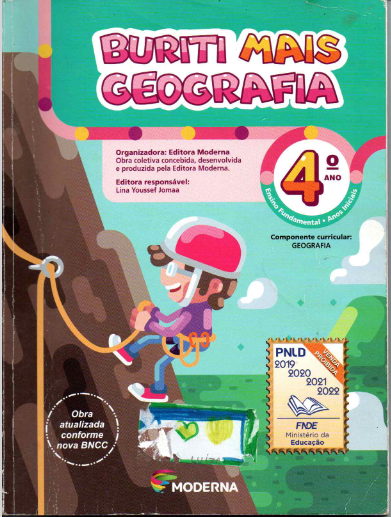
\includegraphics[width=\textwidth]{Fig1.png}
 \caption{Página 1 do Livro de Geografia “Buriti Mais Geografia – 4ª ano”.}
 \label{fig1}
 \end{minipage}%
 \hfill
 %\qquad
 \begin{minipage}{0.45\textwidth}
 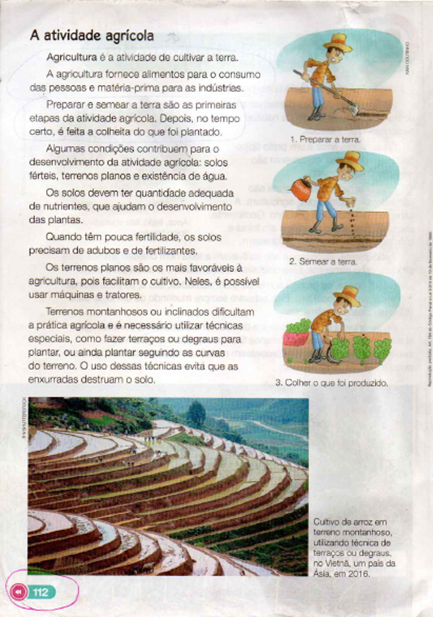
\includegraphics[width=\textwidth]{Fig2.png}
 \caption{Página 2 do Livro de Geografia “Buriti Mais Geografia – 4ª ano”.}
 \label{fig2}
 \end{minipage}% 
 \source{Editora Moderna.}
\end{figure}

\begin{figure}[htbp]
 \centering
 \begin{minipage}{.45\textwidth}
 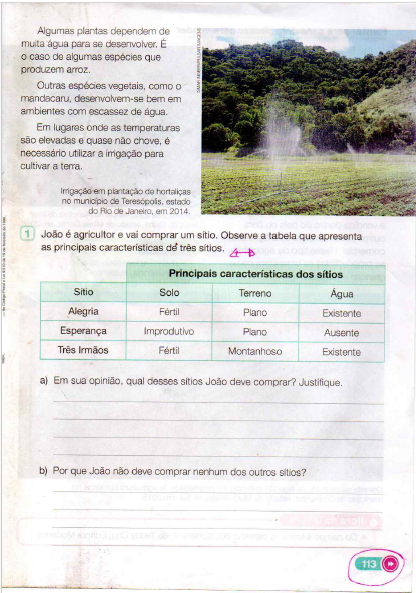
\includegraphics[width=\textwidth]{Fig3.png}
 \caption{Página 3 do Livro de Geografia “Buriti Mais Geografia – 4ª ano”.}
 \label{fig3}
 \end{minipage}%
 \hfill
 \begin{minipage}{0.45\textwidth}
 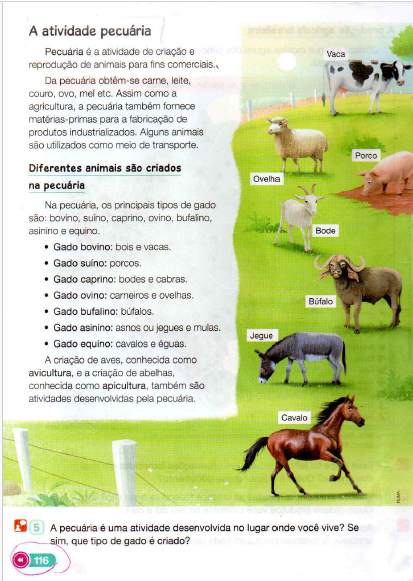
\includegraphics[width=\textwidth]{Fig4.png}
 \caption{Página 4 do Livro de Geografia “Buriti Mais Geografia – 4ª ano”.}
 \label{fig4}
 \end{minipage}% 
 \source{Editora Moderna.}
\end{figure}

Por diversas vezes, fizemos a leitura do capítulo, mas por conta da quantidade de páginas (páginas 111 até 121, ou seja, dez páginas totais), decidimos por selecionar somente as páginas 112, 113 e 116 para a tradução em Libras. O primeiro texto, denominado de “A atividade agrícola”, das páginas 112 e 113, contêm onze parágrafos e cinco figuras. Há, ainda, na página 113, uma atividade, mas a descartamos. Na página 116, há outro texto, denominado de “A atividade pecuária”, contendo seis parágrafos e uma figura que ilustra alguns animais.

Na fase de tradução, realizamos a decupagem do texto em uma tabela, dividindo-a em números correspondentes às cenas em libras e que seriam gravadas pela tradutora surda Rosemeire Aparecida Antunes Desidério. Há, ainda, uma coluna com foco no texto-fonte em português escrito e outra coluna com o texto-alvo em glosas escritas da sinalização em Libras (\Cref{tab02}). 


\needspace{10\baselineskip} % 
\begin{footnotesize}
\renewcommand{\arraystretch}{1.5}
\begin{longtable}{
l 
    >{\raggedright\arraybackslash}p{0.45\textwidth}
    >{\raggedright\arraybackslash}p{0.45\textwidth}
    }
\caption{Fase de tradução.}
\label{tab02}
\\
\toprule
Cenas & Texto-Fonte & Texto-Alvo  \\
 \midrule
001 & \textbf{Agricultura é a atividade de cultivar a terra.} & AGRICULTURA É O QUE? FUNÇÃO ARAR SEMEAR TERRA. \\
002 & A agricultura fornece alimentos para o consumo das pessoas e matéria-prima para as indústrias &
AGRICULTURA DÁ ALIMENTOS PESSOAS VIVER MATERIA+PRIMA PROPRIA INDUSTRIA \\
003 & Preparar e semear a terra são as primeiras etapas da atividade agrícola. Depois, no tempo certo, é feita a colheita do que foi plantado. & PRIMERA (DEDO) APONTAR AGRICOLA TERRA PREPARAR DEPOIS SEMEAR PASSAR TEMPO COLHER PASSADO O-QUE FOI PLANTADO \\
004 & Algumas condições contribuem para o desenvolvimento da atividade agrícola: solos férteis, terrenos planos e existência de água. & ALGUNS IMPORTANTES AJUDAR DESENVOLVER AREA AGRICOLA COMO: SOLO BOM, TERRA RETA TBM ÁGUA TER. \\
005 & Os solos devem ter quantidade adequada de nutrientes, que ajudam o desenvolvimento das plantas. &
SOLO PRECISA TER NUTRIENTES BOM DESENVOLVER PLANTA. \\
006 & Quando têm pouca fertilidade, os solos precisam de adubos e de fertilizantes. & SE POUCO TERRA BOA SOLO PRECISAR ADUBOS (CL) FERTILIZANTE \\
007 & Os terrenos planos são os mais favoráveis à agricultura, pois facilitam o cultivo. Neles, é possível usar máquinas e tratores. & TERRA RETA AJUDAR A AGRICULTURA, FACIL 

PLANTAR TBM PODER USAR MÁQUINAS TRATOR \\
008 & Terrenos montanhosos ou inclinados dificultam a prática agrícola e é necessário utilizar técnicas especiais, como fazer terraços ou degraus para plantar, ou ainda plantar seguindo as curvas do terreno. O uso dessas técnicas evita que as enxurradas destruam o solo. & TERRA MONTANHA CURVA (TORTA) PRECISA  USAR TECNICA RECURSO (MATERIAL) PROPRIA PLANTAR  USO MATERIAL (RECURSO) EVITAR CHUVA AGUA FORTE DESTRUIR SOLO. \\
009 & Cultivo de arroz em terreno montanhoso, utilizando técnica de terraços ou degraus, no Vietnã, um país da Ásia, em 2016. & PAIS VIETNA ANO 2016 LA TER PLANTAR ARROZ TERRA MONTANHA TORTA \\
010 & Algumas plantas dependem de muita água para se desenvolver. É o caso de algumas espécies que produzem arroz. & PLANTA ALGUM PRECISAR ÁGUA PARA VIVER EXEMPLO ARROZ. \\
011 & Outras espécies vegetais, como o mandacaru, desenvolvem–se bem em ambientes com escassez de água. & OUTRA VEGETAL EXEMPLO MANDACARU PRODUÇÃO LUGAR POUCA AGUA É POSSIVEL. \\
012 & Em lugares onde as temperaturas são elevadas e quase não chove, é necessário utilizar a irrigação para cultivar a terra. & LUGAR TEMPO QUENTE CHOVER POUCO PRECISAR IRRIGAÇÃO PLANTAR TERRA BOA \\
013 & Irrigação em plantação de hortaliças no municípios de Teresópolis, estado do Rio de Janeiro, em 2014. & CIDADE TE-R-E-S-O-P-O-L-I-S ESTADO RIO DE JANEIRO PLANTA HORTA PRECISAR IRRIGAÇÃO \\
014 & \textbf{A atividade pecuária} & PECUARIA \\
015 & Pecuária é a atividade de criação e reprodução de animais para os fins comerciais. & 
PECUARIA FUNÇÃO E PRODUZIR ANIMAIS VENDER \\
016 & Da pecuária obtém-se carne, leite, couro, ovo, mel etc. Assim como a agricultura, a pecuária também fornece matérias-primas para a fabricação de produtos industrializados. & 
AREA PECUARIA VENDER CARNE, LEITE, COURO BOI, OVO, MEL. 

AREA AGRICULTURA AREA PECUARIA DA MATERIA PRIMA FAZER PRODUTOS ALIMENTOS E ALIMENTOS PROPRIO INDUSTRIA. \\
017 & Alguns animais são utilizados como meio de transporte. & ANIMAIS ALGUNS USAR TRABALHO TRANSPORTE PECUARIA \\
018 & \textbf{Diferentes animais são criados na pecuária} & AREA PECUARIA ANIMAIS DIFERENTE CRIAR TER \\
019 & Na pecuária, os principais tipos de gado são: bovino, suíno, caprino, ovino, bufalino, asinino e equino. & TER VARIOS TIPOS

GRUPO PROPRIO (GADO)

EXEMPLO:  GRUPO BOI, GRUPO PORCO,

GRUPO BODE, GRUPO

OVELHAS, GRUPO BUFALO.

GRUPO BURRO, GRUPO CAVALO. \\
020 &
\begin{itemize}
    \item  Gado bovino: bois e vacas
    \item Gado suíno: porcos 
    \item Gado caprino: bodes e cabras
    \item Gado ovino: carneiros e ovelhas
    \item Gado bufalino: búfalos
    \item Gado asinino: asnos ou jegues e mulas.
    \item Gado equino: cavalos e éguas
\end{itemize} &
GRUPO BOI, LEITE 

GRUPO PORCO,

GRUPO BODE,

GRUPO OVELHAS,

GRUPO BUFALO,

GRUPO BURRO,

GRUPO CAVALO   FEMEA  \\
021 & A criação de aves, conhecida como avicultura, e a criação de abelhas, conhecida como apicultura, também são atividades desenvolvidas pela pecuária. & NA AREA A-V-I-C-U-L-T-U-R-A CONHECER NOME   

GRUPO PASSARO ( AVES)  TAMBEM CONHECER A-P-I-C-U-L-T-U-R-A PRODUZIR  PECUARIA \\
022 & A pecuária é uma atividade desenvolvida no lugar onde você vive? Se sim, que tipo de gado é criado? & 
LUGAR ONDE VOCE MORA TER PECUARIA? SE SIM TIPO DE GRUPO ( GADO ) QUAL? \\
\bottomrule
\source{Elaborada pelos autores.}
\end{longtable}
\end{footnotesize}


Rosemeire fez as gravações de vídeos-rascunhos remotamente, com usos de baixas tecnologias. Em seguida, estes materiais passaram pela revisão de Glauber Lemos, com foco linguístico e verificação das aplicações de técnicas tradutórias. O nosso objetivo principal, com a tradução, era incorporar as categorias de Descrição Imagética da libras. A gravação final foi feita na residência de Rosemeire, em São Paulo. No vídeo, podemos perceber que há uma parede com fundo liso e de cor azul clara e gelo. Foram utilizados outros materiais tecnológicos, tais como: lâmpada \textit{Ring Light}; iluminador de anel, contendo luz de 16cm e 6 polegadas; tripé de mesa. 

A edição foi feita pelo aplicativo \textit{Microsoft Clipchamp} e incluímos imagens do livro, imagens selecionadas por nós e legendas do texto escrito em português. O processo de gravação demorou três dias, com o total de 18 horas de dedicação da tradução até a execução da edição e inclusão da legendagem. Foram gravados 22 vídeos, totalizando, assim, 12 minutos e 53 segundos de texto-vídeo. A tradução pode ser assistida por este link: \url{https://youtu.be/_GKc-8xqWos?si=ZowKrcWvtTr-FIRp}\footnote{Ressaltamos que este dado de pesquisa é o resultado da tradução de uma aluna surda e que estudou em um curso de especialização, portanto, os dados são oriundos do processo final de sua aquisição tradutória em libras. Não queremos, aqui, medir ou verificar profunda habilidade e fluência tradutória.}.

Apresentamos, nas subseções seguintes, alguns trechos de nossa proposta de tradução, aplicando as incorporações de descritores imagéticos \cite{campello2008visualidade}, usos de técnicas tradutórias como equivalência e adaptação do texto-fonte para o texto-alvo e o processo tradutório intersemiótico em libras.

\subsection{Tradução em libras com uso de descritor imagético de Transferência de Tamanho e Forma (TTF)}\label{sec-modelo}
Para realizarmos a tradução do trecho abaixo nos deparamos com uma palavra que não conseguimos encontrar uma equivalência em libras: mandacaru. Assim, realizamos pesquisas por meio de uma imagem que pudesse representar a referida planta e, em seguida, fizemos estudos de suas características principais. 

Verificamos que o mandacaru é uma planta nativa da região nordestina e que consegue sobreviver a temperaturas altas e por muito tempo. Em outra busca, focamos em textos traduzidos em libras. Também procuramos por glossários no Youtube, que pudessem conter um possível sinal de mandacaru. Assim, encontramos o canal de autoria de Matheus Anacleto\footnote{Link do canal: Mandacaru, cardeiro, jamacaru, mãdaka'ru ou iamanaka'ru (Cereus jamacaru) (youtube.com)}. O sinal MANDACARU (\Cref{fig5}), assim como realizado por Matheus Anacleto, foi incorporado em nossa tradução, pois apresentava as características da planta, possuindo espinhos, folhagens endurecidas e ressecadas, além de incorporar, respectivamente, seu tamanho e sua forma. 

\begin{figure}[h!]
    \centering
    \begin{minipage}{0.25\linewidth}
    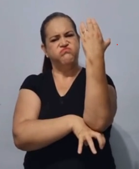
\includegraphics[width=\linewidth]{Fig5.png}
    \caption{Sinal de MANDACARU.}
    \label{fig5}
    \source{Dos autores.}
    \end{minipage}
\end{figure}

Para que conseguíssemos inserir em nossa tradução a descrição imagética de transferência de forma e tamanho \cite{campello2008visualidade}, utilizamos a incorporação icônica do formato bem enrijecido do Mandacaru, com uso de expressão facial e corporal. Neste trecho, decidimos pela adaptação no texto-alvo. 

Com a decisão por utilizar o sinal de Mandacaru, apresentamos um trecho de nossa tradução em libras do texto de geografia (\Cref{fig6}).

\begin{figure}[h!]
    \centering
    \begin{minipage}{0.85\linewidth}
    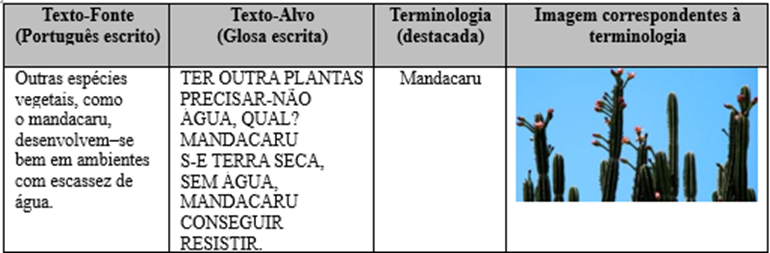
\includegraphics[width=\linewidth]{Fig6.png}
    \caption{Tradução em libras do texto de geografia.}
    \label{fig6}
    \source{Elaboração própria.}
    \end{minipage}
\end{figure}

A imagem acima, com foco na sinalização realizada em 05:39.39, descreve a transferência de forma da planta MANDACARU, ilustrando icônica e imageticamente a resistência do vegetal, sem ao menos ter água por um longo período de tempo, além de conseguir produzir flores e frutos. As flores do mandacaru foram sinalizadas e formadas na transferência da sinalização, tanto pequenas, quanto avolumadas. Aqui, a sinalização traduzida retrata, em sua corporeidade-textualidade, como a planta é em seu formato original, além de apresentar todas as características deste vegetal. 

\subsection{Tradução em libras com uso do descritor imagético de Transferência Espacial (TE)}\label{sec-organizacao}
No trecho, a seguir, apresentamos a nossa proposta de tradução em libras, em 03:04.53, com atenção aos termos de “terrenos montanhosos ou inclinados” (\Cref{fig7}).

\begin{figure}[h!]
    \centering
    \begin{minipage}{0.85\linewidth}
    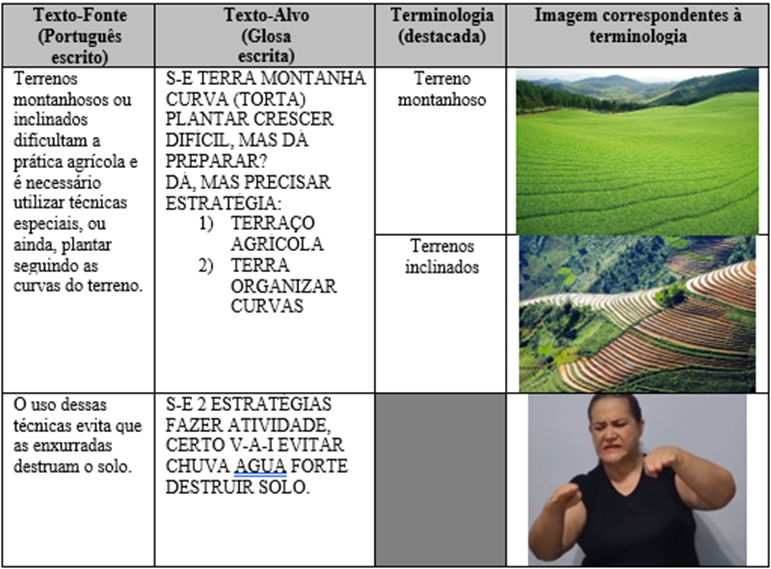
\includegraphics[width=\linewidth]{Fig7.png}
    \caption{Tradução em libras de "terrenos montanhosos ou inclinados”.}
    \label{fig7}
    \source{Elaboração própria.}
     \end{minipage}
\end{figure}

Nesse momento, tivemos que buscar por imagens que trouxessem referências e características de como são organizadas as plantações em espaços montanhosos e com terrenos inclinados. Isso porque, no texto-fonte não havia imagens que relacionassem figura-conceito. Por isso, em uma busca virtual, encontramos algumas opções, mas decidimos por escolher a primeira imagem, contida no quadro acima,  para ser transferida no corpo-texto-sinalizador, correlacionando-a ao conceito de “terreno montanhoso”. Para descrever visualmente um “terreno montanhoso”, observamos que, geralmente, a inclinação deste tipo de terreno não é tão declive, mas, sim, possui leves curvaturas geográficas. Assim, as mãos da sinalizadora buscou manter a regularidade espacial e a angulação de como seria o espaço pelo qual fazia referência visual.

Na segunda imagem, também, contida no quadro acima, em relação aos “terrenos inclinados”, percebemos que é um terreno localizado em um espaço montanhoso, com muitas formas arredondadas e com camadas estratificadas de cima para baixo, como uma escada. Verificamos que, no contexto da plantação, algumas destas curvaturas são feitas pelos agricultores para servirem de plantio a determinadas espécies e vegetações. 

Com o entendimento dessas características imagéticas-visuais, propomos a incorporação de transferência de espaço na sinalização em libras, além de sua forma, para, assim, permitir que os alunos surdos possam compreender visualmente como é feito o plantio nesta região/localização. Dessa forma, é possível que se compreenda visualmente a profundidade espacial, os diferentes ângulos e as diferentes perspectivas, oriundas de uma MONTANHA, contendo plantio de vegetação específica desta localidade.

No trecho sinalizado em 00:05.31, apresentamos o sinal de REGIÃO- AGRICULTURA para dar o sentido de perspectiva e amplitude territorial (\Cref{fig8}).

\begin{figure}[h!]
    \centering
    \begin{minipage}{0.85\linewidth}
    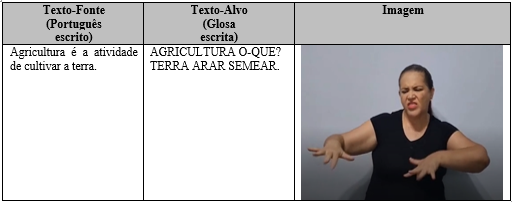
\includegraphics[width=\linewidth]{Fig8.png}
    \caption{Sinal de REGIÃO- AGRICULTURA em Libras.}
    \label{fig8}
    \source{Elaboração própria.}
    \end{minipage}
\end{figure}

Para evitarmos a tradução literal ou palavra-sinal, optamos em realizar a transferência de espaço e, assim, permitir que os surdos compreendam e percebam, por meio da sinalização, como são organizados o território, o trabalho de agricultura e a atividade agropecuária, com foco na semeação de determinada vegetação e no cuidado de animais. Realizamos, recorrentemente, a sinalização da semeação neste mesmo espaço visual para mantermos a coerência visual do texto-vídeo traduzido em língua de sinais. Aqui, o foco linguístico foi estabelecer os referentes espaciais geográficos em libras.

\subsection{Tradução em Libras com uso de descritor imagético de Transferência de Localização (TL)}\label{sec-organizacao-latex}
Tivemos bastante dificuldade para encontrarmos equivalência em libras do termo “matéria-prima”, aliás, o referido termo possui uma definição bem longa, pois são componentes que passam pelo ciclo e processo de manufaturação e fabricação. Em libras, encontramos um glossário terminológico, tematizando “Agronomia, agropecuária e horticultura”\footnote{Link do canal \url{https://www.youtube.com/playlist?list=PL-QJfwj7mJ4x9ncUG-9BGpzg8MBj5XMxp}}, tendo sido elaborado pelo Instituto Federal do Rio Grande do Sul (IFRS), no entanto, não havia nenhum sinal-termo de “matéria-prima”. Em outra busca realizada no Youtube, encontramos o canal de “Tatils Libras”, apresentando uma proposta de sinal para “matéria-prima”\footnote{Link do canal \url{https://www.youtube.com/watch?v=YLOJEPsIm58}}. 

Decidimos que o trecho do texto-fonte que tivesse o conceito de “matéria-prima” precisaríamos utilizar a técnica tradutória mais explicativa, com foco em “AGRICULTURA DÁ ALIMENTOS PESSOAS VIVER MATERIA+PRIMA PROPRIA INDUSTRIA”. Em nossa tradução, o sentido de matéria-prima se concentrou em apresentar materiais que eram plantados e cresciam, ocasionando, assim, na colheita (\Cref{fig9}).

\begin{figure}[h!]
    \centering
    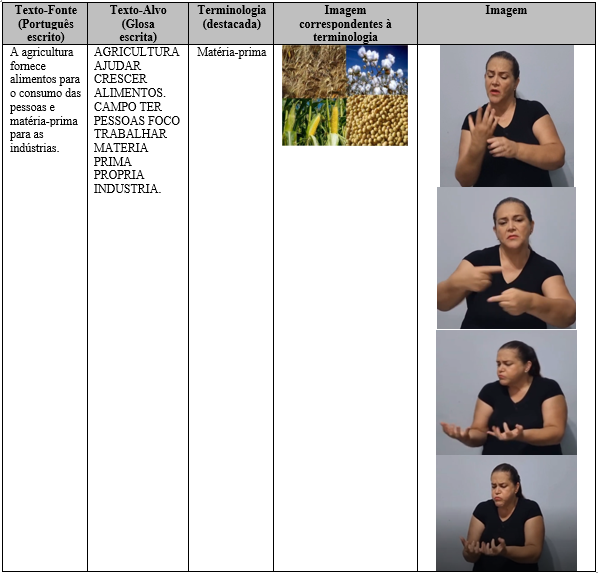
\includegraphics[width=0.75\linewidth]{Fig9.png}
    \caption{Tradução de “AGRICULTURA DÁ ALIMENTOS PESSOAS VIVER MATERIA+PRIMA PROPRIA INDUSTRIA” em Libras.}
    \label{fig9}
    \source{Elaboração própria.}
\end{figure}

Para mantermos a coerência da sinalização em libras, buscamos fixar o local da sinalização, posicionando o mesmo ponto que se referenciava à produção agrícola. Assim, a tradutora surda incorporou a expressão facial, de bochecha inflada, para se referenciar ao sinal de CRESCER e, dessa maneira, descrever imageticamente a transferência de localização-espacial. Com isso, buscamos apresentar o sentido da intensidade linear e, também, a incorporação icônica-visual da germinação, realizada pelo agricultor. Inserimos na tradução em libras, a ação do crescimento da semente no corpo-texto-sinalizador, na mesma localização e direcionalidade.

\subsection{Tradução em libras com uso de descrito imagético de Transferência de Movimento (TM)}\label{sec-titulo}
Na minutagem 00:07:00, a sinalização de ARAR busca incorporar a transferência imagética de movimento, dando ênfase à visualidade em libras. Consideramos que não era necessário que o tradutor realizasse a tradução literal de cada palavra-sinal, referindo-se a “PEGAR ENXADA BATER TERRA DEPOIS ARAR”. Ou seja, com o uso de apenas um sinal de ARAR na sinalização e utilizando a descrição imagética, foi possível transferir todas as ações e seus respectivos movimentos na tradução em Libras (\Cref{fig10}).

\begin{figure}[h!]
    \centering
    \begin{minipage}{0.3\linewidth}
    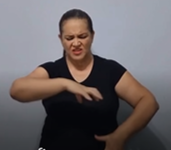
\includegraphics[width=\linewidth]{Fig10.png}
    \caption{Sinal ARAR.}
    \label{fig10}
    \source{Dos autores.}
    \end{minipage}
\end{figure}

A transferência de movimentação de ARAR se repetiu, causando recorrência visual (de direita para a esquerda) em todo o texto-vídeo em Libras. Acreditamos que esta repetição do movimento e em determinada localização pode permitir que o aluno surdo compreenda como ocorre a sequencialidade de uma atividade agrícola, com foco em arar, plantar, regar, crescer e colher. Assim, os alunos surdos podem entender que o movimento de arar faz parte da ecologia de trabalho do cultivo em terra, além de correlacioná-lo com a imagem que faz referência a atividade.

Na minutagem de 00:10:55, apresentamos a sinalização de SEMEAR, realizando, aqui, a descrição imagética de transferência de movimento em junção à transferência espacial, com foco em “SEMEAR ABRIR BURACO, COLOCAR SEMENTE”. As sequencialidades das ações, descritas visualmente, permitem que os alunos surdos compreendam como é feita a produção agrícola e que há similaridades das ações nas atividades agrícolas (\Cref{fig11}).

\begin{figure}[h!]
    \centering
    \begin{minipage}{.3\textwidth}
    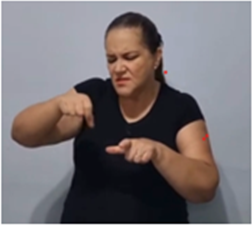
\includegraphics[width=\linewidth]{Fig11.png}
    \caption{Sinal SEMEAR.}
    \label{fig11}
    \source{Dos autores.}
    \end{minipage}
\end{figure}

Neste trecho traduzido, a proposta da sinalização é de se referir a um espaço e que o leitor-visual possa compreender que uma determinada pessoa planta sementes e de forma linear. Aqui, é possível explicitar a movimentação da sinalização e de forma detalhada e clara, permitindo, assim, que os alunos surdos compreendam o texto de geografia, traduzido em libras.

\subsection{Tradução em libras com uso de descritor imagético de Transferência de Incorporação (TI)}\label{sec-idioma}
No trecho abaixo, apresentamos como a tradutora surda incorporou os objetos e as ações da agricultura em sua sinalização em libras (\Cref{fig12}). 

\begin{figure}[h!]
    \centering
    \begin{minipage}{.85\textwidth} 
    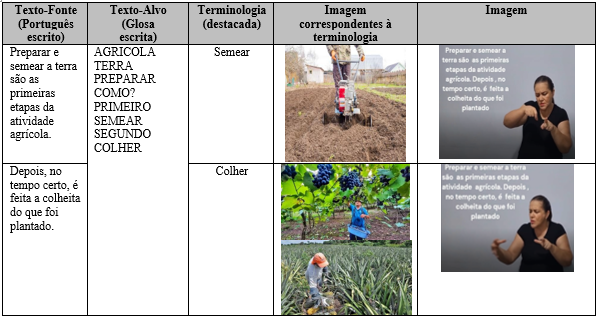
\includegraphics[width=\linewidth]{Fig12.png}
    \caption{Incorporação dos objetos e das ações da agricultura por tradutora surda em libras.}
    \label{fig12}
    \source{Dos autores.}
    \end{minipage}
\end{figure}

Para realizarmos a tradução destes dois trechos, primeiramente, decidimos por aglutiná-los e deixar a mensagem-conteúdo mais claro possível para os alunos surdos. Em seguida, buscamos por imagens que se referenciassem às ações do agricultor, tais como SEMEAR e COLHER. Em seguida, em nossa proposta de tradução em libras, no trecho 00:49.60, há o apontamento de como o agricultor, utilizando determinada ferramenta para ARAR a terra e, também, para cultivar o plantio. Na sinalização, acima destacada, buscamos diferenciar a direcionalidade das ações de SEMEAR e COLHER, incorporando, ainda, de forma linear e reta, a abertura de buracos para ocorrer o lançamento das sementes, de forma contínua, além de incorporar as ações de germinação e colheita do plantio. Todas essas ações são incorporadas no corpo-texto-sinalizador, apresentando os movimentos e as sensações do trabalho realizado por um agricultor.

Conforme a sinalização realizada em 01:26.17, também, destacamos as ações que descrevem a incorporação e o movimento do objeto que irriga as plantações, o aspersor e/ou bombas de tubulações em um espaço com vegetação que precisa de constante irrigação (\Cref{fig13}). 

\begin{figure}[h!]
\centering
\begin{minipage}{0.5\textwidth}
    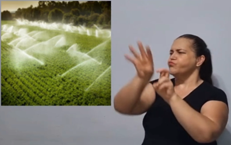
\includegraphics[width=\linewidth]{Fig13.png}
    \caption{Sinal IRRIGAR.}
    \label{fig13}
    \source{Dos autores.}
\end{minipage}
\end{figure}


A tradutora surda incorpora os objetos, por exemplo, como as tubulações, em diferentes ângulos, jorrando a água e em um espaço de cultivo. Aqui, buscamos realizar uma tradução mais criativa, com inserção da técnica de transferência de incorporação, para, assim, encenar, imageticamente, como a ÁGUA JORRAR-LADOS e permitir que o sentido de IRRIGAR ocorra em movimentos curvilíneos e com uso de expressão facial e de bochechas infladas. 

Neste trecho, traduzido em texto-vídeo em libras, a tradutora surda constrói o significado de como ocorre o fornecimento e controle da água, apresentando, ainda, como as plantas são tratadas e como se utilizam as máquinas agrícolas para realizar a irrigação de determinada plantação. 

Acreditamos que os alunos surdos, quando assistirem a este texto-vídeo traduzido em libras, possam compreender cada ação referente à agricultura e à agropecuária, além dos trabalhos rurais e cuidados com a vegetação. 

\section{Conclusão}\label{sec-resumo}
Nesta pesquisa realizamos uma proposta de tradução em texto-vídeo em libras para o público-alvo de alunos surdos, com idade em torno de nove e dez anos, correspondendo a um texto de geografia, escrito em português, referente ao 4º ano, do ensino fundamental I. Consideramos que é possível, sim, construir um material didático de geografia traduzido em texto-vídeo em libras. 

Em nossa proposta de tradução de texto de geografia tivemos que realizar escolhas linguísticas e tradutórias, abarcando os usos de elementos descritivos imagéticos da libras (transferências de tamanho/forma, espaço, localização, movimento e incorporação). A tradutora surda realizou a incorporação icônica-visual verbal e não verbal em seu corpo-texto-sinalizador e apontamento visual e manual para as imagens incluídas no texto-vídeo. Com os usos descritores na sinalização foi possível manter a recorrência visual e transferir os sentidos referentes aos sinais e às imagens. Buscamos pesquisar imagens para além do que se tinha no texto-fonte e, assim, suscitar a iconicidade e criatividade na tradução, descrevendo em detalhes as ações do ciclo dos vegetais, das atividades da agricultura e do cuidado com a terra, ou seja, as ações da agricultura (arado, plantação, semeação, irrigação e colheita).

Os dados analisados apontam que os usos das descrições imagéticas na sinalização em libras permitem deixar a tradução em texto-vídeo mais coerente e adequada para o nosso público-alvo, os alunos surdos. Ou seja, a nossa proposta de texto-vídeo em libras abarcou os usos de elementos visuais, imagens, legendas e o corpo-texto-sinalizador de uma tradutora surda, construindo, assim, o sentido de um discurso sinalizado adequado, com usos de aspectos visuais e o respeito à cultura surda. Assim sendo, a nossa tradução é avessa a tradução literal de palavra-sinal, pois optamos pela tradução intersemiótica, tanto entre signos verbais e não verbais, quanto entre signos verbais-orais-auditivos e signos verbais-espaciais-visuais, com foco no sentido, na criatividade e na transformação.

Por fim, acreditamos que se os professores e as instituições escolares/universitárias utilizarem as traduções em textos-vídeos em libras e se permitirem a propor a produção de outros materiais didático-escolares bilíngues em libras, com foco em conteúdos e textos de geografia, conseguirão fomentar um processo de ensino-aprendizagem para os alunos surdos mais atrativo, informativo e sociocultural.


\printbibliography\label{sec-bib}
% if the text is not in Portuguese, it might be necessary to use the code below instead to print the correct ABNT abbreviations [s.n.], [s.l.]
%\begin{portuguese}
%\printbibliography[title={Bibliography}]
%\end{portuguese}


%full list: conceptualization,datacuration,formalanalysis,funding,investigation,methodology,projadm,resources,software,supervision,validation,visualization,writing,review
\begin{contributors}[sec-contributors]
\authorcontribution{Glauber de Souza Lemos}[conceptualization,methodology,projadm,validation,supervision,writing,review]
\authorcontribution{Rosemeire Aparecida Antunes Desidério}[datacuration,investigation,visualization,writing]
\end{contributors}


\end{document}


